\begin{lstlisting}
//ENUMERATIONS +++++++++++++++++++++++++++++++++++++++++++++++++++

enum ApplicationStatus { LastEvaluation, Rejected, Screening, OnlineAssessment, Accepted }
enum QuestionType { MultipleChoice, OpenQuestion, TrueOrFalse }
enum InternshipDuration { TwoToThreeMonths, ThreeToSixMonths, SixToTwelveMonths, MoreThanOneYear }
enum AnswerStatus {Completed, Uncompleted}

//SIGNATURE +++++++++++++++++++++++++++++++++++++++++++++++++++


abstract sig User{
    email: disj one Email,
    password: disj one Password
}

sig Student extends User{
	cv: disj one CV,
	appliedTo: Internship,
	skills: some Skills,
	feedback_of_internship: Internship -> some Feedback,
	feedback_of_platform: Feedback,
	enrolled: one University
 }

sig University extends User{
	tracked_internship : Student -> Internship,
	tracked_feedback : Internship -> Feedback,
	feedback_of_internship : Feedback -> Internship
}{this in Student.enrolled}


sig Company extends User {
    	feedback_of_internship: Feedback -> Internship,
	feedback_of_platform: Feedback
}

sig Internship{
	suitable_skills: set Skills,
	feedback_internship: disj set Feedback,
	questions: set Internship_Question,
	applications: disj set Student -> Application
}

sig Application{
	title: String,
	description: String,
	status: ApplicationStatus,
	forInternship: one Internship,
	answers: set Answer
}

sig Internship_Question{
	has_questions: set Question,
}{this in Internship.questions}

sig Match{
	match: Student -> some Internship
}

sig Skills{}


sig Question {
	answer: disj one Answer,
	type: QuestionType
}{this in Internship_Question.has_questions}

sig Answer {
	completed: one Bool
}

sig Feedback {}

sig Email {}
sig Password {}

sig CV {
}{this in Student.cv}


enum Bool {True, False}

//FACT
//++++++++++++++++++++++++++++++++++++++++++//

fact ApplicationMustHaveStatus{
	all a: Application |
		one a.status
}


//Match between student and internship needs to have the same preferences
fact SameMatchSamePreferences{
	all m: Match | all s: Student | all i: Internship |
		s->i in m.match iff #(s.skills & i.suitable_skills) != 0
}



//Intersection between match and application must be empty
fact MatchAndApplicationDisjoint {
    all s: Student, i: Internship|
        (s -> i in Match.match) implies not (i in (s.appliedTo))
}


//A student cannot apply to the same application more than one time
fact MaximumOneApplicationPerIntership{
	all s : Student
| no i : Internship | i in (s.appliedTo) and #(i & (s.appliedTo)) > 1
}


//Internship question must be a subset of question
fact InternshipQuestionsSubset {
    all iq: Internship_Question | iq.has_questions in Question
}

//In order to have an Accepted_Application all answer must be completed
fact AllAnswersMustBeCompletedForAcceptedApplication {
	all i: Internship| all q: Question| all s: Student |
	s.((i.applications).status) in Accepted implies q in i.questions.has_questions and q.answer.completed in True
}

//The answer are available only in an Accepted_Application status
fact AnswersOnlyInAcceptedApplication {
    all i: Internship, s: Student | 
        some i.questions.has_questions implies s.((i.applications).status) in Accepted
}


//Application has feedback only if its status is either Accepted_Application or Rejected_Application
fact FeedbackOnlyForAcceptedOrRejectedApplication {
    all s: Student | all i: Internship |
        some i.(s.feedback_of_internship) implies s.((i.applications).status) in Accepted or s.((i.applications).status) in Rejected
}


//Cannot add feedback to application which are not Accepted_Application
fact NoFeedbackForNonAcceptedApplication {
    all i: Internship, s: Student |
        some i.feedback_internship implies (s.(i.applications).status) in Accepted
}

//PREDICATES
//+++++++++++++++++++++++++++++++++++++++++++++++++++++++++++++++++++

//User add a CV
pred StudentAddCV[s: Student, cv_new: CV]
{
	s.cv = s.cv + cv_new
} 

//User remove a CV
pred StudentRemoveCV[s: Student, cv_to_remove: CV]
{
	s.cv = s.cv - cv_to_remove
}

//New Match has been found between a student and internship and added
pred AddNewMatch(s: Student, i: Internship, m: Match) {
    s -> i in m.match
    and s.skills & i.suitable_skills != none
}

//New feedback for an internship has been added by a student
pred NewFeedbackStudent[f_new: Feedback, s: Student, i: Internship]
{
    i.(s.feedback_of_internship) = i.(s.feedback_of_internship) + f_new
}

//New feedback has been added by a company
pred NewFeedbackCompany[f_new: Feedback, c: Company, i: Internship]
{
    (c.feedback_of_internship).i = (c.feedback_of_internship).i + f_new
}

//Every student's feeback must be tracked by his university
fact UniversityTracksFeedback {
    all s: Student, i: Internship, u: University |
        some i.(s.feedback_of_internship) implies i.(u.tracked_feedback) = i.(s.feedback_of_internship)
}

// Ensure the university tracks internships for students who have provided feedback
fact UniversityTracksInternships {
    all s: Student, i: Internship, u: University |
        some i.(s.feedback_of_internship) implies i in s.(u.tracked_internship)
}



//ASSERTION +++++++++++++++++++++++++++++++++++++++++++++++++++

assert FeedbackConsistency {
    all i: Internship | all s: Student |  all u: University |
    (i in (s.appliedTo) and #(i.(s.feedback_of_internship)) != 0) implies 
     i.(u.tracked_feedback) = i.(s.feedback_of_internship) and i in s.(u.tracked_internship)
}

assert ValidMatch {
    all m: Match | all s: Student | all i: Internship |
    s -> i in m.match implies s.skills & i.suitable_skills != none
}


pred simpleWorld{
	#Student = 1
	#University = 1
	#Company = 1
	#Internship = 2
	#Internship_Question = 1
	#Question = 1
	#Skills = 1
}

//TO RUN ASSERTION AND PREDICATES

run StudentAddCV for 4

run StudentRemoveCV for 4

run AddNewMatch for 4

run NewFeedbackStudent for 4

run NewFeedbackCompany for 4

check FeedbackConsistency

check ValidMatch

run simpleWorld for 5


\end{lstlisting}



\begin{figure}
    \centering
    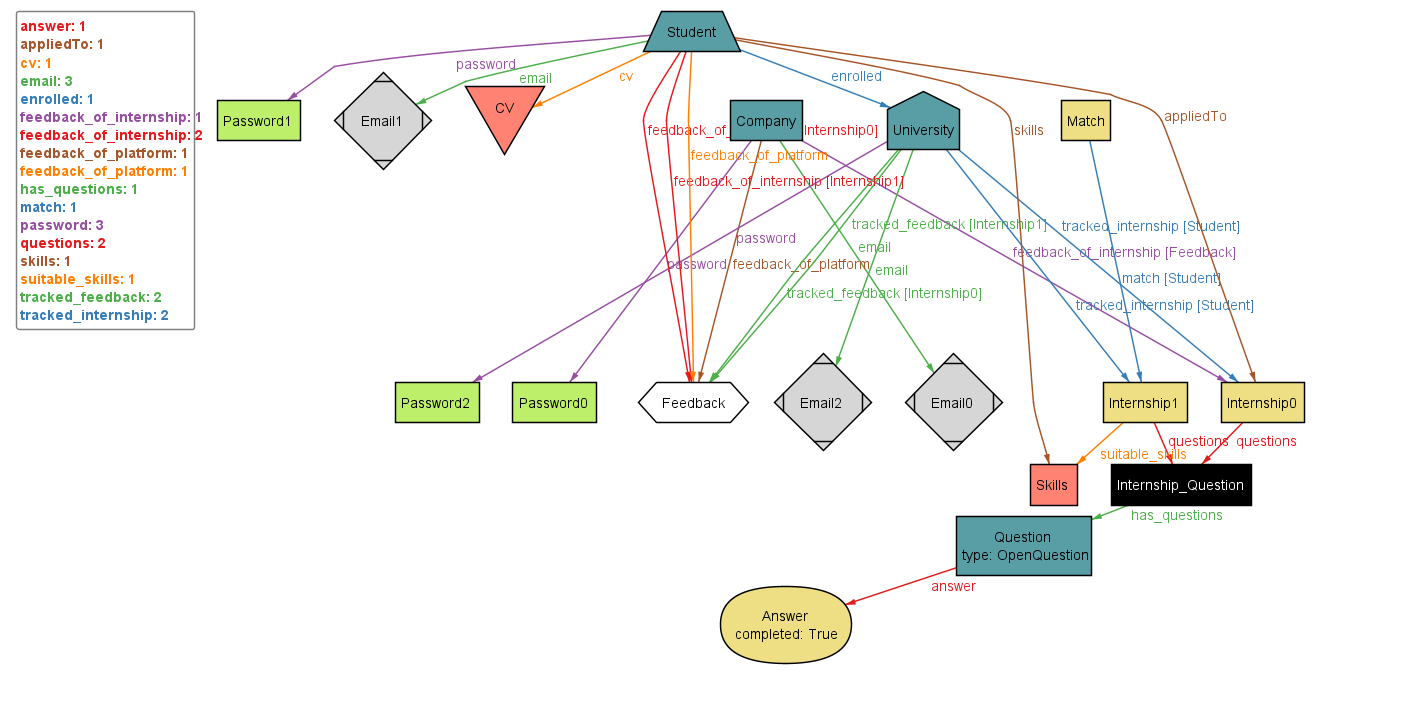
\includegraphics[angle=270, width=0.65\linewidth]{Images/ImagesRASD/AlloySimpleWorld.png}
    \caption{Simple world description in Alloy}
    \label{fig:simple-world}
\end{figure}



\pagebreak
